% slides v5 — synced to paper (Apr 25, 2026): headline 1.11deg temporal, 40% reduction,
% LOYO 1.26 +/- 0.19 deg, along-track 1D snapshot caveat. Overflow-guarded.
\documentclass[aspectratio=169,11pt]{beamer}
\usetheme{default}
\usecolortheme{dove}
\setbeamertemplate{navigation symbols}{}
\setbeamertemplate{footline}[frame number]
\setbeamerfont{frametitle}{size=\large,series=\bfseries}
\setbeamercolor{frametitle}{fg=darkblue}
\definecolor{darkblue}{RGB}{27,58,92}
\definecolor{medblue}{RGB}{41,128,185}
\usepackage{graphicx}
\usepackage{booktabs}
\usepackage{tikz}
\usepackage{array}
\usepackage{caption}
\captionsetup{labelformat=empty}

\title{Predicting the Ionospheric Cusp Location from Solar Wind}
\subtitle{An XGBoost Model Trained on 27 Years of DMSP Data}
\author{Yiwen~Zhu \and Adam~T.~Michael \and Frank~R.~Toffoletto}
\institute{Rice University \& JHU/APL}
\date{}

\begin{document}

%% 1: Title
\begin{frame}[plain]
\titlepage
\vspace{-0.4cm}
\centering\small Submitted to \emph{JGR: Space Physics} (under review, manuscript 2026JA035567)
\end{frame}

%% 2: What is the Cusp
\begin{frame}{What is the Cusp?}
\begin{columns}[T]
\begin{column}{0.55\textwidth}
\begin{itemize}
\item Narrow funnel near each magnetic pole where solar wind plasma enters the magnetosphere along open field lines
\item DMSP at $\sim$840~km sees a 1--2\textdegree{} MLAT band of low-energy ion precipitation (Newell criteria)
\item Equatorward boundary tracks the dayside reconnection rate
\item Practical impact: GPS scintillation, LEO drag, polar-route aviation radiation
\item No operational model currently predicts cusp location from upstream solar wind
\end{itemize}
\end{column}
\begin{column}{0.42\textwidth}
\centering
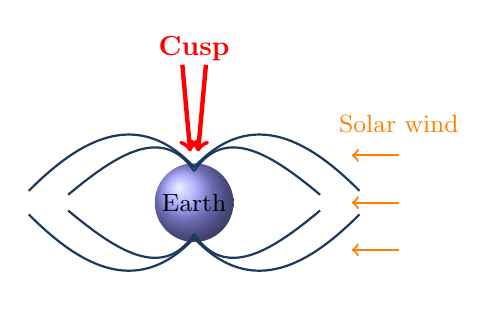
\begin{tikzpicture}[scale=0.50]
  \shade[ball color=blue!40] (0,0) circle (1.0);
  \node at (0,0) {\small Earth};
  \foreach \s in {1,-1} {
    \draw[thick,darkblue] (0,\s*0.9) .. controls (1.5,\s*2.5) and (3,\s*1.5) .. (4.2,\s*0.3);
    \draw[thick,darkblue] (0,\s*0.9) .. controls (-1.5,\s*2.5) and (-3,\s*1.5) .. (-4.2,\s*0.3);
    \draw[thick,darkblue] (0,\s*0.8) .. controls (0.8,\s*2.0) and (2.0,\s*1.2) .. (3.2,\s*0.2);
    \draw[thick,darkblue] (0,\s*0.8) .. controls (-0.8,\s*2.0) and (-2.0,\s*1.2) .. (-3.2,\s*0.2);
  }
  \draw[red,ultra thick,->] (-0.3,3.5) -- (-0.1,1.3);
  \draw[red,ultra thick,->] (0.3,3.5) -- (0.1,1.3);
  \node[red,font=\bfseries] at (0,3.9) {Cusp};
  \foreach \y in {-1.2,0,1.2} {
    \draw[->,thick,orange] (5.2,\y) -- (4.0,\y);
  }
  \node[orange,font=\small] at (5.2,2.0) {Solar wind};
\end{tikzpicture}
\end{column}
\end{columns}
\end{frame}

%% 3: Prior Models
\begin{frame}{Where Existing Models Stand}
\begin{itemize}
\item \textbf{Newell et al.\ 2006}: 10 coupling functions tested. Best ($E_{WAV}$): $r \approx 0.56$ on individual crossings, $0.81$ on binned data. 60-min averaging beats instantaneous.
\item \textbf{Newell \& Sotirelis 2007}: universal coupling function $d\Phi_{MP}/dt$. $r = 0.85$ binned.
\item \textbf{Anderson \& Bukowski 2024}: 41k DMSP crossings; tilt slope varies with MLT and IMF $B_y$ sign.
\item \textbf{Global MHD}: faithful but hours of CPU per run; not operational.
\end{itemize}
\vspace{0.3cm}
\textbf{The gap}: every published predictor uses 1--2 SW parameters and linear / low-order nonlinear fits. Crossing-to-crossing scatter is large ($r \sim 0.56$--$0.58$). Multi-parameter ML has not been applied.
\end{frame}

%% 4: Data
\begin{frame}{Data --- DMSP + OMNI}
\begin{columns}[T]
\begin{column}{0.50\textwidth}
\begin{itemize}
\item \textbf{DMSP F06--F18}, 1987--2014 (27 yr $\approx$ 2.5 solar cycles)
\item SSJ/4 + SSJ/5 spectrometers, 1-s cadence
\item Anderson cusp criteria $\to$ \textbf{39{,}668 crossings} (clean, AE-filtered)
\item Along-track boundaries: eq/pole MLAT + eq/mean MLT at the satellite's MLT
\item \emph{This is a 1D snapshot at one MLT, not the full 2D cusp}
\end{itemize}
\vspace{0.2cm}
\small\textbf{OMNI L1}: 1-min IMF + SW $\to$ \textbf{74 features} including 15/30/60-min mean/std/$\Delta$ history
\end{column}
\begin{column}{0.48\textwidth}

\includegraphics[width=\linewidth]{../../figures/fig01_data_coverage.png}
\end{column}
\end{columns}
\end{frame}

%% 5: Feature Table
\begin{frame}{Input Features (74 Total)}
\centering
\footnotesize
\begin{tabular}{l c >{\raggedright\arraybackslash}p{8.0cm}}
\toprule
Category & \# & Key features \\
\midrule
Geometry        & 3  & dipole tilt, hemisphere, day-of-year \\
Raw IMF         & 3  & $B_x$, $B_y$, $B_z$ \\
Solar wind      & 3  & $v$, $n$, $P_\mathrm{dyn}$ \\
Coupling        & 7  & $d\Phi_{MP}/dt$, $E_{KL}$, $vB_s$, $B_T$, $\theta_c$, $B_y\cdot\mathrm{sgn}(\text{hemi})$, $\sin(\theta_c/2)$ \\
15-min history  & 18 & mean, std, $\Delta$ of 6 IMF/SW vars \\
30-min history  & 18 & mean, std, $\Delta$ of 6 IMF/SW vars \\
60-min history  & 22 & mean, std, $\Delta$ + integrals of $d\Phi_{MP}/dt$, $vB_s$ \\
\midrule
\textbf{Total}  & \textbf{74} & \\
\bottomrule
\end{tabular}
\vspace{0.3cm}

\normalsize Key choice: include time-integrated history because the magnetosphere takes $\sim$1~hr to reconfigure after an IMF change.
\end{frame}

%% 6: Method
\begin{frame}{Method --- XGBoost on Tabular SW $\to$ Cusp}
\begin{itemize}
\item \textbf{XGBoost}: gradient-boosted decision trees. 1000 trees, depth 8, lr 0.02, subsample 0.8, colsample 0.7.
\item Tree models beat NNs on tabular data (Grinsztajn et al.\ 2022); we confirmed against MLP, ResMLP, TabTransformer.
\item Targets (multi-output): eq MLAT, pole MLAT, eq MLT, mean MLT.
\item Interpretability: gain importance + SHAP + partial dependence.
\end{itemize}
\vspace{0.2cm}
\centering
\resizebox{0.78\textwidth}{!}{%
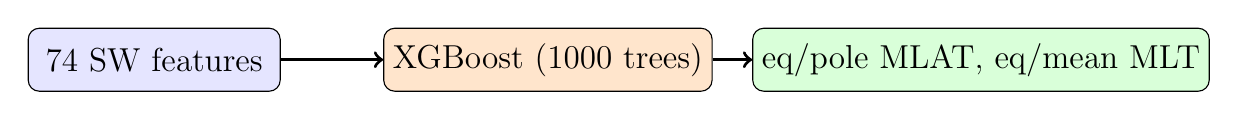
\begin{tikzpicture}
  \node[draw,fill=blue!10,rounded corners,minimum width=3.2cm,minimum height=0.8cm,font=\large]
    (inp) at (0,0) {74 SW features};
  \node[draw,fill=orange!20,rounded corners,minimum width=3.2cm,minimum height=0.8cm,font=\large]
    (xgb) at (5,0) {XGBoost (1000 trees)};
  \node[draw,fill=green!15,rounded corners,minimum width=3.8cm,minimum height=0.8cm,font=\large]
    (out) at (10.5,0) {eq/pole MLAT, eq/mean MLT};
  \draw[->,very thick] (inp) -- (xgb);
  \draw[->,very thick] (xgb) -- (out);
\end{tikzpicture}}
\end{frame}

%% 7: Headline Results
\begin{frame}{Headline Result --- Temporal Holdout}
\begin{columns}[T]
\begin{column}{0.52\textwidth}

\includegraphics[width=\linewidth]{../../figures/fig02_scatter_4panel.png}
\end{column}
\begin{column}{0.45\textwidth}
\footnotesize
\textbf{Train pre-2008 / test 2008--2014}
\vspace{0.15cm}
\begin{tabular}{lccc}
\toprule
Target & MAE & $R^2$ & $r$ \\
\midrule
eq MLAT (\textdegree)   & \textbf{1.11} & 0.79 & 0.89 \\
pole MLAT (\textdegree) & 1.09 & 0.79 & 0.89 \\
eq MLT (hr)             & 0.77 & 0.48 & 0.70 \\
mean MLT (hr)           & 0.73 & 0.49 & 0.71 \\
\bottomrule
\end{tabular}
\vspace{0.3cm}

\textbf{1.11\textdegree{} $\approx$ 122~km on the dial}\\
$\approx$60\% of crossings within 1\textdegree, 90\% within 2\textdegree

\vspace{0.2cm}
\small Random-split (paper-1 backup): MAE = 0.97\textdegree.
\end{column}
\end{columns}
\end{frame}

%% 8: Robustness — LOYO + Baseline
\begin{frame}{Generalization \& Baseline Comparison}
\begin{columns}[T]
\begin{column}{0.52\textwidth}

\includegraphics[width=\linewidth]{../../figures/fig03_baseline_comparison.png}
\end{column}
\begin{column}{0.45\textwidth}
\footnotesize
\textbf{Leave-one-year-out (23 years):}
\begin{itemize}
\item MAE = $1.26 \pm 0.19$\textdegree
\item Robust across solar cycle phases
\end{itemize}
\vspace{0.15cm}
\textbf{vs.\ baselines (temporal holdout):}
\begin{tabular}{lcc}
\toprule
Method & MAE & $r$ \\
\midrule
Linear ($B_z$)        & 2.04\textdegree & 0.39 \\
Linear (Newell CF)    & 1.85\textdegree & 0.58 \\
Nonlinear Newell      & 1.80\textdegree & 0.59 \\
\textbf{XGBoost}      & \textbf{1.11\textdegree} & \textbf{0.89} \\
\bottomrule
\end{tabular}
\vspace{0.3cm}

\textbf{40\% MAE reduction} over best linear baseline\\
\small $p<0.001$
\end{column}
\end{columns}
\end{frame}

%% 9: Error Distribution
\begin{frame}{Error Distribution}
\begin{center}

\includegraphics[width=0.80\textwidth]{../../figures/fig04_error_distribution.png}
\end{center}
{\footnotesize Residuals: mean $< 0.03$\textdegree{} (near-zero bias), std $\approx 1.34$\textdegree.\quad
Multi-crossing within-group spread $\sim$1.03\textdegree{} $\Rightarrow$ model MAE approaches the natural cusp variability floor.}
\end{frame}

%% 10: Feature Importance
\begin{frame}{What the Model Learned}
\begin{columns}[T]
\begin{column}{0.55\textwidth}

\includegraphics[width=\linewidth]{../../figures/fig05_feature_importance.png}
\end{column}
\begin{column}{0.42\textwidth}
\footnotesize
\textbf{Top predictors:}
\begin{itemize}
\item \textbf{\#1} ($\sim$31\%): 60-min mean $d\Phi_{MP}/dt$
\item \textbf{\#2} ($\sim$11\%): 60-min mean $vB_s$
\item \#3--4 ($\sim$6\% each): 60-min integrals of $d\Phi_{MP}/dt$, $vB_s$
\item Hemisphere ($\sim$5\%), dipole tilt ($\sim$2\%)
\end{itemize}
\vspace{0.2cm}
60-min $\gg$ 30-min $>$ 15-min $\gg$ instantaneous
\vspace{0.2cm}

\textbf{Model rediscovered the established physics on its own.}
\end{column}
\end{columns}
\end{frame}

%% 11: Time-Window Ablation
\begin{frame}{How Much History Matters?}
\begin{columns}[T]
\begin{column}{0.55\textwidth}

\includegraphics[width=\linewidth]{../../figures/fig06_time_window_comparison.png}
\end{column}
\begin{column}{0.42\textwidth}
\footnotesize
\begin{tabular}{lc}
\toprule
Feature set & MAE \\
\midrule
Instantaneous only      & 1.27\textdegree \\
+ 15-min history        & 1.08\textdegree \\
+ 30-min history        & 1.02\textdegree \\
+ 60-min history        & 0.99\textdegree \\
All windows combined    & \textbf{0.97\textdegree} \\
\bottomrule
\end{tabular}
\vspace{0.3cm}

\normalsize 60-min history gives the single largest gain ($-0.20$\textdegree).\\[4pt]
Matches the $\sim$1-hr magnetospheric reconfiguration timescale.
\end{column}
\end{columns}
\end{frame}

%% 12: Partial Dependence
\begin{frame}[shrink=2]{Physical Relationships --- Partial Dependence}
\begin{center}

\includegraphics[width=0.74\textwidth]{../../figures/fig07_partial_dependence.png}
\end{center}
{\footnotesize (a) Dipole tilt slope $-0.05$\textdegree/\textdegree{} (Newell 1989).\ (b) Newell CF nonlinear saturation.\ (c) $B_z$ asymmetry.\ (d) $P_{dyn}$.\ (e) $B_y$.\ (f) $vB_s$.\ Each panel recovers a known empirical relationship without being told the formula.}
\end{frame}

%% 13: Model Architecture Comparison
\begin{frame}{XGBoost vs.\ Neural Networks}
\begin{columns}[T]
\begin{column}{0.54\textwidth}

\includegraphics[width=\linewidth]{../../figures/fig09_model_comparison.png}
\end{column}
\begin{column}{0.42\textwidth}
\footnotesize
\begin{tabular}{lcc}
\toprule
Model & MAE & Train \\
\midrule
Linear (Newell)    & 1.83\textdegree & 0.1~s \\
GBR-300            & 1.11\textdegree & --   \\
\textbf{XGBoost}   & \textbf{0.97\textdegree} & 80~s \\
\midrule
MLP-GeLU           & 1.54\textdegree & 11~s \\
ResMLP             & 1.01\textdegree & 36~s \\
TabTransformer     & 1.11\textdegree & 136~s \\
\bottomrule
\end{tabular}
\vspace{0.3cm}

\normalsize Tree models beat NNs on this tabular task (Grinsztajn et al.\ 2022).
\end{column}
\end{columns}
\end{frame}

%% 14: Hemispheric + Geomagnetic Activity
\begin{frame}{Robustness: Hemisphere \& Activity}
\begin{columns}[T]
\begin{column}{0.55\textwidth}

\includegraphics[width=\linewidth]{../../figures/fig10_hemi_ae.png}
\end{column}
\begin{column}{0.42\textwidth}
\footnotesize
\textbf{Hemisphere} (random split):\\
N ($n\approx$7180, 90\%): MAE 0.93\textdegree\\
S ($n\approx$754, 10\%): MAE 1.29\textdegree
\vspace{0.2cm}

\textbf{Geomagnetic activity (AE):}
\begin{tabular}{lc}
\toprule
AE level & MAE \\
\midrule
Quiet ($<$100)       & 0.96\textdegree \\
Moderate (100--300)  & 0.92\textdegree \\
Active (300--500)    & 0.94\textdegree \\
Storm ($\geq$500)    & 1.16\textdegree \\
\bottomrule
\end{tabular}
\vspace{0.2cm}

\normalsize Storm: $+25\%$ MAE; still well below the 1.83\textdegree{} linear baseline.
\end{column}
\end{columns}
\end{frame}

%% 15: Limitations, Operations, Take-Home
\begin{frame}{Limitations \& Operational Path}
\begin{columns}[T]
\begin{column}{0.48\textwidth}
\textbf{Scope of the claim:}
\begin{itemize}
\item Along-track 1D boundary at the satellite's MLT
\item Not a full 2D cusp map (work in progress)
\item AE-filtered crossings (Anderson 2024 criterion)
\item 1987--2014 only; rare extremes under-represented
\end{itemize}
\vspace{0.2cm}
\textbf{Real-time path:} all 74 inputs are derivable from upstream L1 monitors (ACE/DSCOVR). Requires validation on real-time L1 data.
\end{column}
\begin{column}{0.48\textwidth}
\textbf{Take-home:}
\begin{itemize}
\item First ML cusp predictor: \textbf{1.11\textdegree{}} temporal holdout, $1.26 \pm 0.19$\textdegree{} LOYO
\item 40\% MAE reduction over best linear baseline
\item Model rediscovered known physics: 60-min Newell CF dominance, dipole tilt slope, CF saturation
\item Path to real-time forecasting from L1 SW monitors
\end{itemize}
\vspace{0.3cm}
\small\textbf{Data \& code}: Zenodo DOI \texttt{10.5281/zenodo.19340792}\\
GitHub: \texttt{YiwenZhu77/cuspML}
\end{column}
\end{columns}
\end{frame}

\end{document}
